Metode \textit{Synthetic Minority Over-sampling Technique} (SMOTE)
\parencite{chawla2002smote} menggunakan pendekatan \textit{over-sampling} yang mana
kelas minoritas ditambah dengan membuat sampel sintetis, bukan dengan
mengganti sampel dari kelas mayoritas menjadi kelas minoritas.
Sampel sintetis dibuat lewat aplikasi dengan beroperasi pada
ruang fitur.
Kelas minoritas ditambah dengan mengambil setiap sampel-sampel dari kelas
minoritas dan membuat sampel sintetis di antara segmen garis yang menghubungkan
setiap $k$ tetangga terdekat (\textit{k-nearest-neighbors}, KNN) dari kelas
minoritas.
Instan dari KNN dipilih secara acak, bergantung dari jumlah
\textit{over-sampling} yang dibutuhkan.

\begin{figure}[htbp]
\centering
\setlength\fboxsep{4pt}
\fbox{
	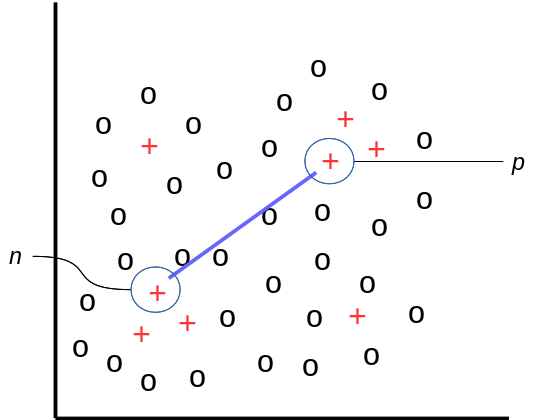
\includegraphics[keepaspectratio=true,scale=0.35]{SMOTE-example}
}
	\caption{
	Ilustrasi pembuatan sampel sintetis pada SMOTE.
	Misalkan $p$ adalah sampel minoritas dan $n$ adalah salah satu dari $k$
	tetangga terdekat dari $p$, maka
	sampel sintetis yang baru akan berada di garis antara $p$ dan $n$.
	}
	\label{fig:smote}
\end{figure}

Sampel sintetis dibuat dengan cara berikut, misalkan $p$ adalah salah satu
sampel minoritas pada dataset $D$,
\pagebreak
\begin{itemize}
	\item Cari $k$ sampel tetangga dari $p$ pada $D$
	\item Untuk setiap sampel tetangga $k$,
	\begin{itemize}
		\item Hitung selisih antara vektor fitur $p$ dengan tetangga $k_{i}$
		\item Kalikan selisih tersebut dengan angka ril acak antara 0 sampai 1,
		dan
		\item simpan hasilnya ke vektor fitur sintentis yang baru.
	\end{itemize}
\end{itemize}

Cara ini membuat sampel secara acak pada segmen garis antara dua fitur yang
terpilih, seperti yang terlihat pada gambar \ref{fig:smote}.
Pendekatan ini secara efektif mendorong wilayah pembelajaran dari kelas
minoritas menjadi lebih besar tanpa menyebabkan \textit{overfitting}.
